\documentclass[journal,11pt,twocolumn]{IEEEtran}
\usepackage[portuguese]{babel}
\usepackage[utf8]{inputenc}
\usepackage[dvips]{graphicx}
\usepackage{amsmath,amsfonts,amssymb}
\usepackage{makecell}
\usepackage[normal]{subfigure}
\usepackage{array,colortbl}
\usepackage{amsmath}
\usepackage{mathrsfs}
\usepackage[sort]{cite}
\usepackage[none]{hyphenat}
\usepackage{minted}
\usepackage{url}
\usepackage[section]{placeins}


% Those packages were originally here, but I don't think we are gonna need them, so I commented them out
%\usepackage[center,small]{caption}
%\usepackage{color}
%\usepackage{colortbl}
%\usepackage{comment}
%\usepackage{float}
%\usepackage{flushend}
%\usepackage[mathfrak]{mathpi}
%\usepackage{morefloats}
%\usepackage{multicol}
%\usepackage{multirow}
%\usepackage{psfrag}
%\usepackage{rangecite}
%\usepackage{tabularx}
%\usepackage{threeparttable}

\graphicspath{ {images/} }
\setminted{breaklines=true}

\sloppy
\newcommand{\goodgap}{%
\hspace{\subfigtopskip}%
\hspace{\subfigbottomskip}}
\newcounter{mytempeqncnt}

\begin{document}

% paper title
\title{Projeto I: Caracteriza\c{c}\~{a}o de canais banda estreita}


\author{Vinícius Dantas de Lima Melo
    \thanks{Este trabalho foi como parte do curso de Comunicações Móveis oferecido pelo Departamento de Engenharia de Comunicações da UFRN.}
}

% The paper headers
\markboth{Nome do Evento}{Nome do Evento}

% make the title area
\maketitle

\begin{abstract}
Esse trabalho realiza a decomposição dos efeitos de perda de potência em um sinal em relação à distância entre o transmissor e o receptor. Os dados analisados foram gerados sinteticamente e, portanto, a abordagem descrita é de engenharia reversa. Tenta-se, então, encontrar os parâmetros de descrição do canal ao separar os diferentes efeitos de perda sobre o sinal.
\end{abstract}

\begin{keywords}
Caracterização de canal, aderência estatística, desvanecimento, sombreamento.
\end{keywords}

%\IEEEpeerreviewmaketitle

\section{Introdução}
Caracterização de canais de comunicação é uma tarefa extremamente importante para tornar possível simulações e prototipagem. Embora haja momentos em que simulações e protótipos se encontrem, essa possível reproducibilidade faz com que se possa analisar e depurar problemas, reduzindo os custos relacionados a suas correções e respectivos testes. 

Contudo, uma onda eletromagnética propagando-se está sob efeito de diversos fenômenos físicos. Sendo assim, além de analisar as perdas de potência como um todo, deve-se analisar e conhecer-se os diferentes efeitos que estão influenciando nesse comportamento.

\subsection{Proposta do Trabalho}
Observando-se um sinal inventado, aplicar-se-á uma regressão linear em conjunto com um filtro passa-baixa para separar os diferentes componentes do sinal. Isolando-os devidamente e para melhor caracterização, utilizar-se-á um teste de aderência estatística para modelar as perdas que apresentam comportamento não-determinístico.

\subsection{Metodologia}
Para as análises dos sinais dados, foram-se utilizadas simulações e cálculos feitos em scripts em Python utilizando as bibliotecas Numpy (versão 1.16.2) e Scipy (versão 1.2.1) para computação científica e Matplotlib (versão 3.0.3) para plotagem. Os scripts rodaram sobre o interpretador padrão do Python 3.7.1, sobre o qual foram feitos todos os testes, embora espera-se que ele rode sem problema em interpretadores a partir da versão 3.6, pois faz uso de interpolação literal de strings, adicionada nessa versão a partir da PEP 498~\cite{fstrings}.

Utilizando o submódulo stats da biblioteca Scipy, realizou-se o teste de Kolmogorov-Smirnov (KS) de aderência estatística. A partir desse submódulo, teve-se disponível uma variedade de 88 tipos de variáveis aleatórias contínuas para usar no teste de KS, que trabalha com a hipótese nula de que as amostras seguem a distribuição testada\cite{kstest}. O algoritmo implementado para rodar o teste contra essas possibilidades de variáveis aleatórias foi feito de forma a utilizar o paralelismo disponibilizado pela biblioteca multiprocessing, que faz parte da biblioteca padrão do Python, de forma que ele é escalável para o número de CPUs (virtuais ou físicos) disponíveis no computador.

A biblioteca Scipy também disponibiliza outros dois tipos de teste de aderência: o teste de Anderson-Darling~\cite{anderson} e o teste de divergência de potência~\cite{power_divergence}. Contudo, o primeiro só suporta quatro tipos de variáveis aleatórias para executar o teste (normal, exponencial, logísticica e Gumbel), enquanto o teste de divergência de potência trabalha no domínio da frequência ao invés do domínio original do sinal.

Os números reais foram aqui representados com uma precisão de dois algarismos significativos em suas partes decimais.

\section{Análise dos sinais}
Todas as análise foram feitas utilizando o código disponibilizado junto com o artigo e disponível em um repositório git hospedado do Github, disponível através do link \url{https://github.com/viniciusd/DCO1020---Mobile-Communications/tree/master/assignment1}.

Vale salientar que o filtro passa-baixa utilizado, o filtro de médias móveis, foi implementado de forma que apresentasse o mesmo comportamento do disponibilizado por padrão no Matlab. Essa versão não causa descarte de amostras. Para obter um sinal filtrado com o mesmo tamanho do sinal original, esse algoritmo, gradativamente, diminui o tamanho da janela para que seja possível aplicá-la sobre o restante do sinal, conforme descrito em ~\cite{movmean}.

Em contra-partida, para estimar a perda de percurso, foi utilizado o método dos mínimos quadrados para resolução de equações matriciais ~\cite{lstsq}. Esse algoritmo, embora simples, tornou possível que se pudesse seguir fielmente a representação linear no espaço do logaritmo das distância, já que:

\begin{equation*}
    pathLoss = P_{0} + 10nlog_{10}\left(\frac{d}{d_{0}}\right)
\end{equation*}

Utilizando uma equação matricial, pôde-se fixar o valor do intercepto em $P_{0}$. Sendo assim, foi possível obter o coeficiente angular utilizando:

\inputminted[linenos=true]{python}{code/pathloss.py}

Aonde as variáveis prx representam a potência medida no receptor e logdistance é um vetor das distâncias no espaço logarítmico, i.e., $log_{10}\left(\frac{d}{d_{0}}\right)$.

De onde tem-se que o coeficiente de perda de percurso é $n = -\frac{m}{10}$.
\subsection{Sinal simulado}
Foi-nos dado valores de um sinal simulado com o objetivo de que, dado o sinal, conseguíssemos estimar os componentes/efeitos de perda presentes.

Na figura \ref{fig:trial1-original}, podemos obervar como tais componentes se apresentaram. Comparando-a, então, com a figura \ref{fig:trial1-estimated}, observamos um comportamento bem próximo, principalmente da perda de percurso. Quanto ao desvanecimento em larga escala (estimado utilizando um filtro de médias móveis com uma janela de 100 amostras), percebemos que não atingiu as mesmas amplitudes que atingira no sinal simulado, embora tenha apresentado o mesmo comportamento à medida que a distância entre o receptor e o transmissor aumentou.

\begin{figure}[h!]
    \centering
    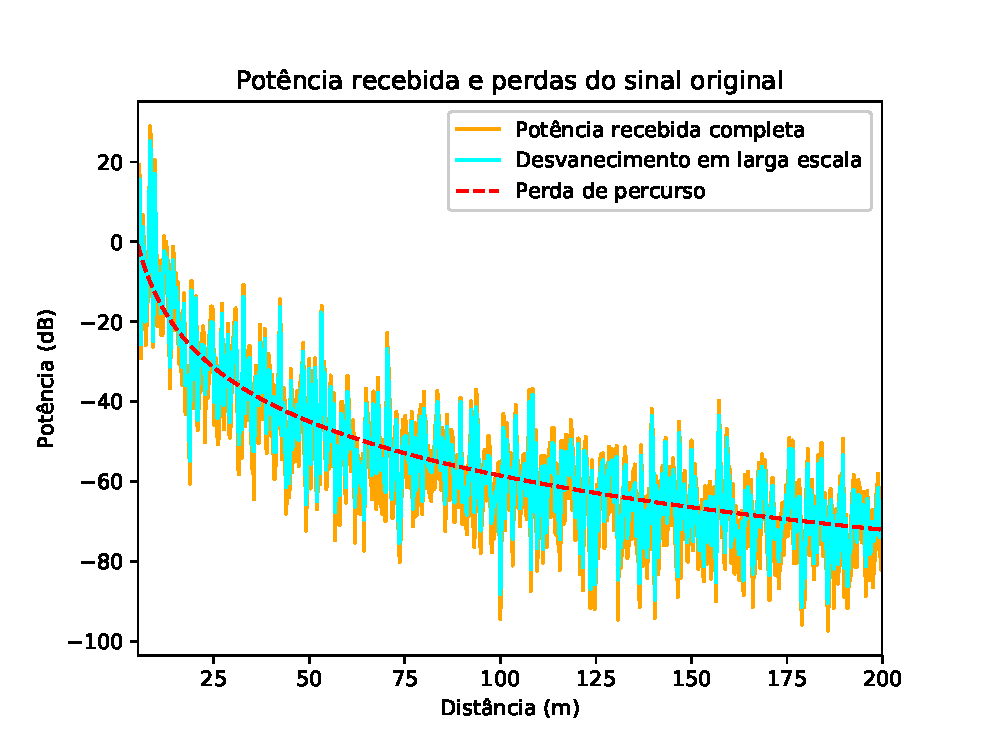
\includegraphics[scale=0.55]{trial1_original.eps}
    \caption{Potência do sinal simulado e seus respectivos componentes de perda ao longo da distância}
    \label{fig:trial1-original}
\end{figure}
\begin{figure}[h!]
    \centering
    \includegraphics[scale=0.55]{trial1_estimated.eps}
    \caption{Potência do sinal estimado e seus respectivos componentes de perda ao longo da distância}
    \label{fig:trial1-estimated}
\end{figure}
Na figura \ref{fig:trial1-pathloss}, podemos observar uma comparação apenas do fenômeno de perda de percurso comparado entre o sinal simulado e o sinal estimado. A partir dessa figura, podemos observar que a estimativa apresenta um comportamento muito próximo ao da curva original.
\begin{figure}[h!]
    \centering
    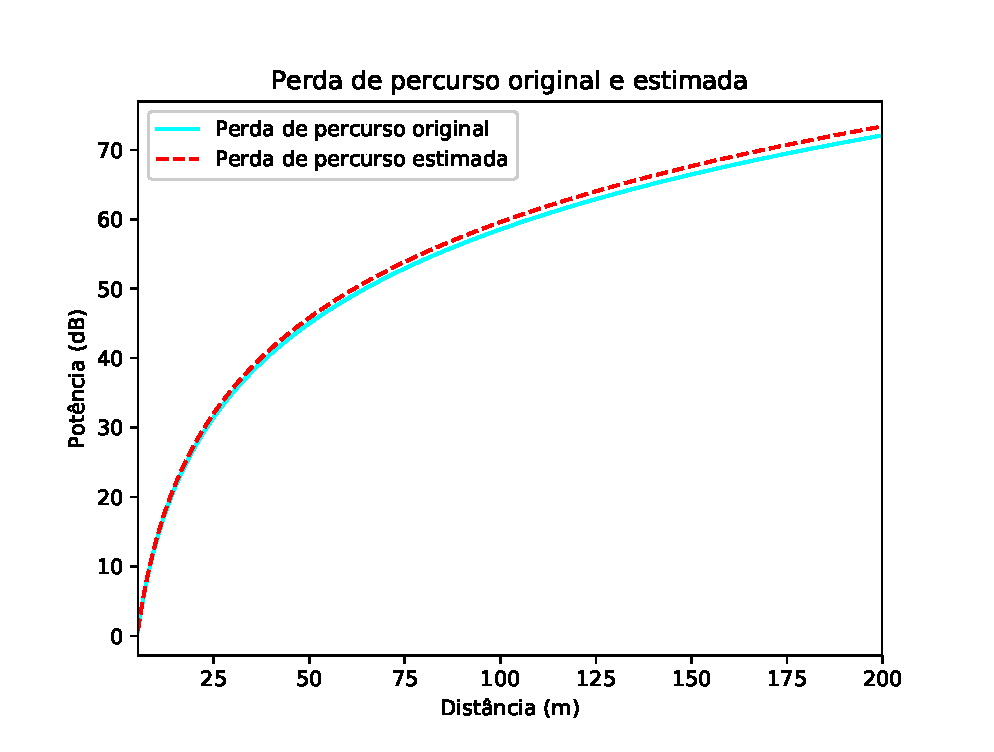
\includegraphics[scale=0.55]{trial1_pathloss.eps}
    \caption{Potência da perda de percurso estimada ao longo da distância}
    \label{fig:trial1-pathloss}
\end{figure}
Outro fenômeno que causa grande degradação da potência é o sombreamento. Podemos observá-lo de forma comparativa na figura \ref{fig:trial1-shadowing}. Aonde podemos confirmar a hipótese de que, embora as curvas não se sobreponham completamente, apresentam o mesmo comportamento e diferem por pequenos valores de amplitude.

Deve-se pontuar, contudo, que o sinal estimado do sombreamento passou por mais uma etapa de adequação: o sombreamento teve sua média movida para zero de forma que não afetasse sua potência. A técnica utilizada para deslocar a média do sombreamento é bem simples e consiste de deslocar o sinal de acordo com a média para movê-la para zero e compensar a perda de potência adicionando uma senóide de frequência arbitrária, a qual não subiria novamente a média.

Essa transformação pode pode ser vista na equação \ref{move-mean-to-0}, aonde $y'$ representa o novo sinal, $y$ o sinal original, $\mu_{y}$ sua média e $x[n]$ sua respectiva abcissa. Quaquer valor de f pode ser utilizado para definir a frequência do senóide, embora seja mais adequado utilizar valores baixos porque frequências altas descaracterizariam o comportamento do sombreamento, já que seriam mais adequadas para o desvanecimento em pequena escala.

\begin{equation}
    y'[n] = y - \mu_{y} + \mu_{y}\cdot seno(2\cdot \pi \cdot f \cdot x[n])
    \label{move-mean-to-0}
\end{equation}
\begin{figure}[h!]
    \centering
    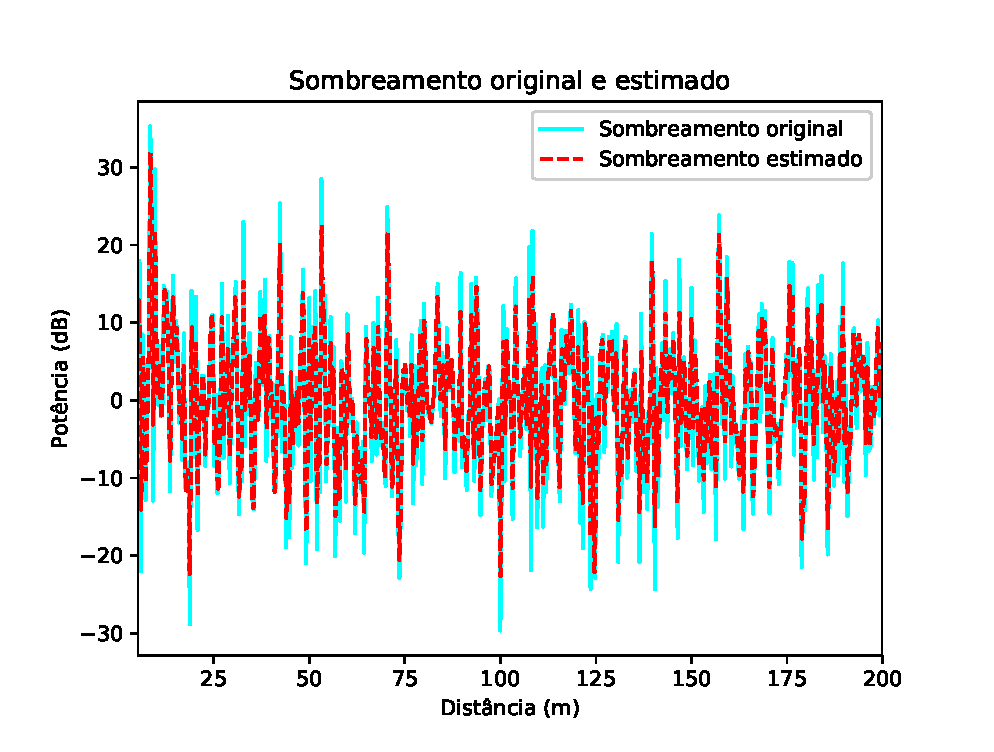
\includegraphics[scale=0.55]{trial1_shadowing.eps}
    \caption{Potência do sombreamento ao longo da distância}
    \label{fig:trial1-shadowing}
\end{figure}
A tabela \ref{tab:shadowing} sumariza algumas medidas para outros valores de janela para o filtro das médias móveis, já que os gráficos anteriores foram feitos com um valor fixo de 100 amostras.

Vale ressaltar que o tamanho da janela não causa efeito no coeficiente de perda de percurso, o que já era esperado porque a perda de percurso foi estimada com base em uma regressão linear do sinal original, o qual não foi afetado pelo filtro.

Outro valor que se mantém constante é a média do sombreamento. Diferente do sombreamento utilizado nos gráficos, aonde a média foi adaptada para 0, observamos uma média constante de 0.16. Esse efeito era esperado porque o filtro aplicado é um filtro passa-baixa e filtros passa-baixa raramente afetam a componente DC (a média). Filtros dessa família que utilizam a média para remover os componentes de alta frequência não causam qualquer efeito na componente DC do domínio da frequência.

Podemos observar também que, embora o desvio-padrão diminua, o erro médio quadrático passa a aumentar a medida que a quantidade de amostras utilizadas na janela do filtro aumenta. Esse comportamento antagônico é esperado porque um filtro passa-baixa reduz o desvio-padrão ao reduzir as [variações de] amplitude do sinal. Uma quantidade maior de amostras torna o sinal cada mais próximo da média, o que também justifica o aumento do erro em relação ao sinal simulado.
\begin{table}[h!]
    \centering
    \begin{tabular}{r|r|r|r|r}
        Janela & Desvio-padrão & Média & \makecell[r]{Coeficiente\\ de perda de \\ percurso} & \makecell[r]{Erro médio\\quadrático\\ normalizado} \\
        \hline
        10  & 8.07 & 0.16 & 4.58 & 0.01\\
        50  & 7.83 & 0.16 & 4.58 & 0.01\\
        100 & 7.30 & 0.16 & 4.58 & 0.03\\
        150 & 6.67 & 0.16 & 4.58 & 0.10\\
        200 & 6.11 & 0.16 & 4.58 & 0.21
    \end{tabular}
    \caption{Características do sombreamento para diferentes tamanhos de janelas de amostras para o filtro de médias móveis no sinal simulado}
    \label{tab:shadowing}
\end{table}

Uma vez que temos o sombreamento caracterizado para os diferentes cenários, a tabela \ref{tab:small-scale-fading} mostra as variáveis aleatórias contínuas que melhor se encaixaram nesse sinal. Utilizando o teste KS contra 88 distribuições disponíveis na Scipy, observamos que a distribuição mais presente é a distribuição gama.

Nessas distribuições que aderem ao tipo gama, o valor de $\alpha$ se mostrou sempre próximo á média, o que faz sentido porque esse parâmetro de forma faz com que os dois lóbulos (já que temos uma gama dupla, i.e., com dois lóbulos simétricos centrados na média), se aproximem. Esse tipo de distribuição é uma generalização de diversas outras, como a exponencial, chi-quadrada e até mesmo a distribuição normal. Uma vez que ela é uma distribuição mais ampla, justifica-se sua presença para todos os tamanhos de janela.

Essa família de distribuições é bastante utilizada em comunicações móveis e sem fio, como mostrado em \cite{nakagami} ao analisar as medidas realizadas in locco. Porém, também utilizada em artigos mais recentes, como \cite{gamma-mixture}, aonde uma mistura de distribuições gama é utilizada para modelar a SNR de canais sem fio. Enquanto \cite{interference} utiliza uma distribuição Gama para modelar a potência da interferência em linha de visada.

Tanto as distribuições Gama quanto a Cauchy são mencionadas em \cite{shadowing_book} como exemplos de distribuições comuns em ambientes sem fio. Para as maiores janelas de filtragem, essas duas distribuições prevaleceram.

\begin{table}[h!]
    \centering
    \begin{tabular}{r|r|r|r|r}
        Janela & \makecell[r]{Primeira\\ melhor\\PDF} & \makecell[r]{Parâmetros\\da primeira\\melhor PDF} & \makecell[r]{Segunda\\ melhor\\PDF} & \makecell[r]{Parâmetros\\da segunda\\melhor PDF} \\
        \hline
        10  & \makecell[r]{Logística\\generali-\\zada\\tipo I\\(gen-\\logistic)} & \makecell[r]{$\alpha=0.62$\\$\mu=0.91$\\escala $=1.02$} & \makecell[r]{Gama\\dupla\\(dgamma)} & \makecell[r]{$\alpha=1.33$\\$\beta=1$\\$\mu=0$\\escala $=1.31$}\\
        50  & \makecell[r]{Gama\\dupla\\(dgamma)} & \makecell[r]{$\alpha=1.35$\\$\beta=1$\\$\mu=0$\\escala $=1.37$} & \makecell[r]{Logística\\generali-\\zada\\tipo I\\(gen-\\logistic)} & \makecell[r]{$\alpha=0.59$\\$\mu=1.08$\\escala $=1.06$}\\
        100 & \makecell[r]{Gama\\dupla\\(dgamma)} & \makecell[r]{$\alpha=1.32$\\$\beta=1$\\$\mu=0$\\escala $=1.60$} & \makecell[r]{Logística\\generali-\\zada\\tipo I\\(gen-\\logistic)} & \makecell[r]{$\alpha=0.69$\\$\mu=0.87$\\escala $=1.30$}\\
        150 & \makecell[r]{Gama\\dupla\\(dgamma)} & \makecell[r]{$\alpha=1.26$\\$\beta=1$\\$\mu=0$\\escala $=2.09$} & \makecell[r]{Cauchy\\(cauchy)} & \makecell[r]{$\mu=0.17$\\escala $=1.92$}\\
        200 & \makecell[r]{Gama\\dupla\\(dgamma)} & \makecell[r]{$\alpha=1.23$\\$\beta=1$\\$\mu=0$\\escala $=2.70$} & \makecell[r]{Cauchy\\(cauchy)} & \makecell[r]{$\mu=0.15$\\escala $=2.38$}
    \end{tabular}
    \caption{Características do sombreamento para diferentes tamanhos de janelas de amostras para o filtro de médias móveis no sinal simulado}
    \label{tab:small-scale-fading}
\end{table}

\subsubsection{Sinal real}

Após o uso do sinal simulado para que pudéssemos calibrar e chegar a uma versão sólida dos scripts escrito, utilizou-se os mesmos procedimentos e algoritmos no sinal real. O uso do sinal simulado foi importante porque tínhamos acesso aos valores de cada componente de perda para podermos comparar e testar o código escrito à medida em que era desenvolvido.

Como o valor de $P_{0}$ não foi dado para esse sinal, realizou-se uma série de iterações em busca de um valor adequado para esse parâmetro. Após diversos testes, chegou-se ao valor de 45dB para a estimativa de $P_{0}$, parâmetro fundamental para a estimativa da perda de percurso.

Essa perda, assim como uma estimativa do desvanecimento em alrga escala, podem ser observados na figura \ref{fig:real-trial1}. Nesse gráfico, tem-se o sinal de potência recebida claramente seguindo o comportamento da curva de perda de percurso estimada. Além disso, temos uma estimativa do desvanecimento de larga escala. Essa estimativa se mostrou bem próxima ao sinal original devido ao pequeno tamanho da janela de amostras utilizada no filtro de médias móveis. Vale salientar, contudo, que o efeito passa-baixa desse filtro pode ser facilmente observado uma vez que variações altas (picos de alta frequência) foram devidamente suavizados.

\begin{figure}[h!]
    \centering
    \includegraphics[scale=0.55]{trial1_real_world_prx_estimated.eps}
    \caption{Potência do sinal estimado seus respectivos componentes de perda ao longo da distância}
    \label{fig:real-trial1}
\end{figure}

Observando as tabelas \ref{tab:real-shadowing} e \ref{tab:real-small-scale-fading}, podemos verificar as mesmas tendências constatadas no sinal simulado. Temos desvios-padrões decrescentes e a mesma família de distribuições estatísticas: Logística generalizada tipo I, Cauchy e Gama dupla.

\begin{table}[h!]
    \centering
    \begin{tabular}{r|r|r|r}
        Janela & \makecell[r]{Desvio-padrão do\\sombreamento\\estimado} & \makecell[r]{Média do\\ sombreamento\\estimado} & \makecell[r]{Coeficiente\\ de perda de \\ percurso}\\
        \hline
        2  & 5.18 & 0.16 & 1.84\\
        5  & 4.60 & 0.08 & 1.84\\
        10 & 4.10 & 0.16 & 1.84\\
    \end{tabular}
    \caption{Características do sombreamento para diferentes tamanhos de janelas de amostras para o filtro de médias móveis no sinal real}
    \label{tab:real-shadowing}
\end{table}

\begin{table}[h!]
    \centering
    \begin{tabular}{r|r|r|r|r}
        Janela & \makecell[r]{Primeira\\ melhor\\PDF} & \makecell[r]{Parâmetros\\da primeira\\melhor PDF} & \makecell[r]{Segunda\\ melhor\\PDF} & \makecell[r]{Parâmetros\\da segunda\\melhor PDF} \\
        \hline
        2  & \makecell[r]{Logística\\generali-\\zada\\tipo I\\(gen-\\logistic)} & \makecell[r]{$\alpha=0.90$\\$\mu=0.10$\\escala $=1.09$} & \makecell[r]{Cauchy\\(cauchy)} & \makecell[r]{$\mu=-0.05$\\escala $=1.04$} \\
        5  & \makecell[r]{Gama\\dupla\\(dgamma)} & \makecell[r]{$\alpha=1.1$\\$\beta=1$\\$\mu=0.04$\\escala $=2.02$} & \makecell[r]{Cauchy\\(cauchy)} & \makecell[r]{$\mu=0.39$\\escala $=1.49$}\\
        10 & \makecell[r]{Logística\\generali-\\zada\\tipo I\\(gen-\\logistic)} & \makecell[r]{$\alpha=0.43$\\$\mu=2.09$\\escala $=1.23$} & \makecell[r]{Gama\\dupla\\(dgamma)} & \makecell[r]{$\alpha=1.05$\\$\beta=1$\\$\mu=-0.07$\\escala $=2.43$}\\
    \end{tabular}
    \caption{Características do sombreamento para diferentes tamanhos de janelas de amostras para o filtro de médias móveis no sinal real}
    \label{tab:real-small-scale-fading}
\end{table}

\section{Conclusões}
Durante o desenvolvimento desse trabalho, seguiu-se uma sequência gradual de análise de um sinal simulado e de um sinal real. O estudo do sinal simulado no começo foi importante para que os algoritmos escritos pudessem ser validados, uma vez que havia valores [simulados] de referência para testar os resultados obtidos.

Ao examinar os dados gerados a partir das análises realizadas, pudemos perceber uma semelhança no comportamento de ambos os sinais. É de suma importância ressaltar o valor da teoria que embasou esses estudos, uma vez que, mesmo frente a uma medição real, mostrou-se sólida e confiável para realizar estimações de canal.

O comportamento do filtro de médias móveis como filtro passa-baixa confirmou-se ao vermos que os desvios-padrões dos sinais filtrados diminuíram enquanto as médias, no geral, permaneceram as mesmas. Observamos apenas um momento em que a média foi afetada, que está exposto na tabela \ref{tab:real-shadowing}. Esse valor pontual pode ter se dado por causa da precisão de números flutuantes ou por causa do pequeno número de amostras do sinal real (200 amostras).

É importante reiterar que as tendências estatísticas observadas ao analisarmos o sinal simulado também puderam ser observadas no sinal real, mesmo utilizando janelas pequenas e tendo um pequeno número de amostras nesse último. Assim como discorrido em \cite{shadowing_book}, pudemos constatar a importância de distribuições sinuosas, como a Gamma, a logística e a Cauchy, no âmbito das comunicações móveis e na descrição de canais.
\bibliographystyle{IEEEtran}
\bibliography{some_books,some_urls}

\end{document}
